\chapter{Energy consumption}\label{ch:power}
When examining the performance of a computer program, its energy consumption is also a key factor: energy conservation must be taken into account in a world where most of the energy is produced through non renewable resources. Moreover the energy used by the device running the program translates into thermal energy that must be dissipated, further increasing the total energy consumption and imposing severe limitations (e.g. volume occupancy) on the computing systems employing those devices.\\
The semiconductor manufacturing process has been constantly improving during the past 40 years bringing ever smaller transistors inside the processing units, which in turn allowed to have ever increasing performances without a substantial increase in energy consumption. For so long Moore's law stood the test: the number of transistors per chip kept doubling every two years or, equivalently, the transistors size in the chip halved every two years.
Unfortunately we are quickly approaching a probable stop of Moore's law: at the 5 $\unit{nm}$ scale -which will be probably reached in few years- the transistor size is of the same order of few radii of silicon atoms. At that scale the quantum tunneling effect also starts to play a role, making very unlikely that the transistors in the processing units, based on the well known silicon technology, will have smaller scale than 5 $\unit{nm}$. At that point any increase in computational power will require an inevitable electrical power increase for the device to operate.\\
For the above reasons it is very important, and it will be even more, that energy efficient computing is also pursued through carefully designed software besides better hardware.\\
In the following sections we will present the measurement of the energy required to run the KD-tree algorithm described in the previous Chapter on different hardware setups.

\section{Measurement methodology}
The nearest neighbors search is the part of the algorithm contributing the most to the energy consumption. As a matter of fact we shown in the previous Chapter that it makes for almost the $90\%$ of the execution time of the entire algorithm. Moreover we want to compare the energy used by the CPU sequential code, running slower but in principle using less power with respect to the more power intensive GPU code that completes the task significantly faster.\\ 
The quantity we can actually measure are two: the time it takes to run the all nearest neighbors search and the the power used by the device performing the search at a given time.
Since the typical time for a complete search is of only few milliseconds, a single search would not be enough to measure accurately the power used in that small time window. For this reason we repeat the very same search several hundreds of times. The total time elapsed to perform all the reiterations of the search is recorded and then divided by the number of repetitions of the search to have the average time of a single search. During those several repetitions the power used is sampled multiple times to evaluate its values and trend. In the case of the GPU parallel code we decided to exclude from the measurement the time needed to move to and from the GPU memory the data needed for the search and its output. Indeed the memory movement uses a very low amount of energy while taking a relatively significant amount of time, thus it would change significantly the end result of the energy consumption measurement.\\
The run time of the search is measured through \code{cudaEvent}, as used for the performance analysis, while the power measurements is performed through dedicated software (when available) and hardware. The CPU sequential code power usage is evaluated through the use of the software \textit{turbostat} that is available for Intel processor, while the GPU code power usage is monitored by \textit{nvidia-smi} available for Nvidia's GPU.\\
To complement all power measurements we also used a common appliance power meter that can be inserted between the wall electricity wall plug and the device to measure the power usage of the whole system.

\section{Benchmark machine}
Monitoring the power meter we evaluate the baseline power usage of the benchmark machine described in Section \ref{sec:benchmark}, that is the power used by the machine when is powered on, in an idle state and ready to run a program. Sampling the read of the power meter over a period of time yield an average baseline power of $60 \pm 1 \unit{W}$.
We build a KD-tree from $5 \times 10^5$ points generated in a volume with a random uniform distribution, we chose the highest amount of points used in the performance study to represent the worst possible scenario of operation.

\subsection{CPU energy consumption}
While running the all nearest neighbors search repeatedly as explained above we sample both the power meter power usage and \textit{turbostat} readings for the whole CPU package. The sampling of the power meter yields an average of $112 \pm 1 \unit{W}$ resulting in an effective increased power usage of $52 \pm 1 \unit{W}$ while the software \textit{turbostat} only reads $21 \pm 1 \unit{W}$: the two measures are clearly incompatible. We attribute this incompatibility to what the status software is actually monitoring, indeed it only reports the power usage of the CPU chip itself, while the power meter, measuring the whole system drainage, takes into account all the other PC components that may draw up more energy when performing the search than when they are idle (e.g. the power supply unit efficiency, the increase of RAM usage, etc...). Since we want to have the most reliable esteem and since we will consider the energy consumption of the whole GPU board when examining the parallel code, we decide to drop the measurement obtained with \textit{turbostat} in favor of the more conservative measurement of the power meter. The average time recorded to perform the all nearest neighbors search on the CPU with the sequential code is of $1.69 \pm 0.01 \unit{s}$ (the power consumption has been observed to be the same over longer periods). We want to express the resulting energy consumption in term of the amount of Joule necessary to perform a single all nearest neighbors search in a given tree, therefore simply multiplying the average power used by the average yields the result: $88 \pm 2 \unit{J/search}$.

\subsection{GPU energy consumption}
To sample the power usage of the GPU board of the benchmark machine we sample the readings from the power meter and from the software \textit{nvidia-smi}. The average of the power meter samples is $196 \pm 1 \unit{W}$ from which must be subtracted the baseline previously measured, yielding $136 \pm 1 \unit{W}$. The average of the samples from \textit{nvidia-smi} is $135 \pm 1 \unit{W}$, therefore the two measures are in agreement which means that the power monitoring software provided by Nvidia takes into account the whole power usage of the GPU board, which is the measure we are interested in.\\
To verify the consistency of the timing needed to perform an all nearest neighbors search we repeat the measurement varying the number of consecutive searches from 100 up to 1000 increasing each step of 100 times. The timing is indeed constant and we extrapolate the average value of $97 \pm 1 \unit{ms}$ per complete search. The final result for the energy consumption is therefore of: $13 \pm 1 \unit{J/search}$.

\section{NVIDIA Tegra K1}
The Tegra K1 (TK1) is a System-on-a-Chip (SoC) developed by NVIDIA featuring an ARM Cortex A15 CPU and a Kepler GPU with 192 CUDA cores.  We where able to test the KD-tree algorithm on this chip mounted on a development board provided by NVIDIA. Picture \ref{tk1_photo} shows the board along with the power meter setup we used to measure the power consumption performance of this board.\\
NVIDIA claims that the TK1 chip is able to deliver excellent performance and power efficiency, for this reason we repeat the same measurement performed for the benchmark machine on this board, evaluating both the ARM CPU capabilities and the integrated GPU's. Unfortunately on this board no power usage monitoring software is available, making the power meter the only option.

\begin{figure}
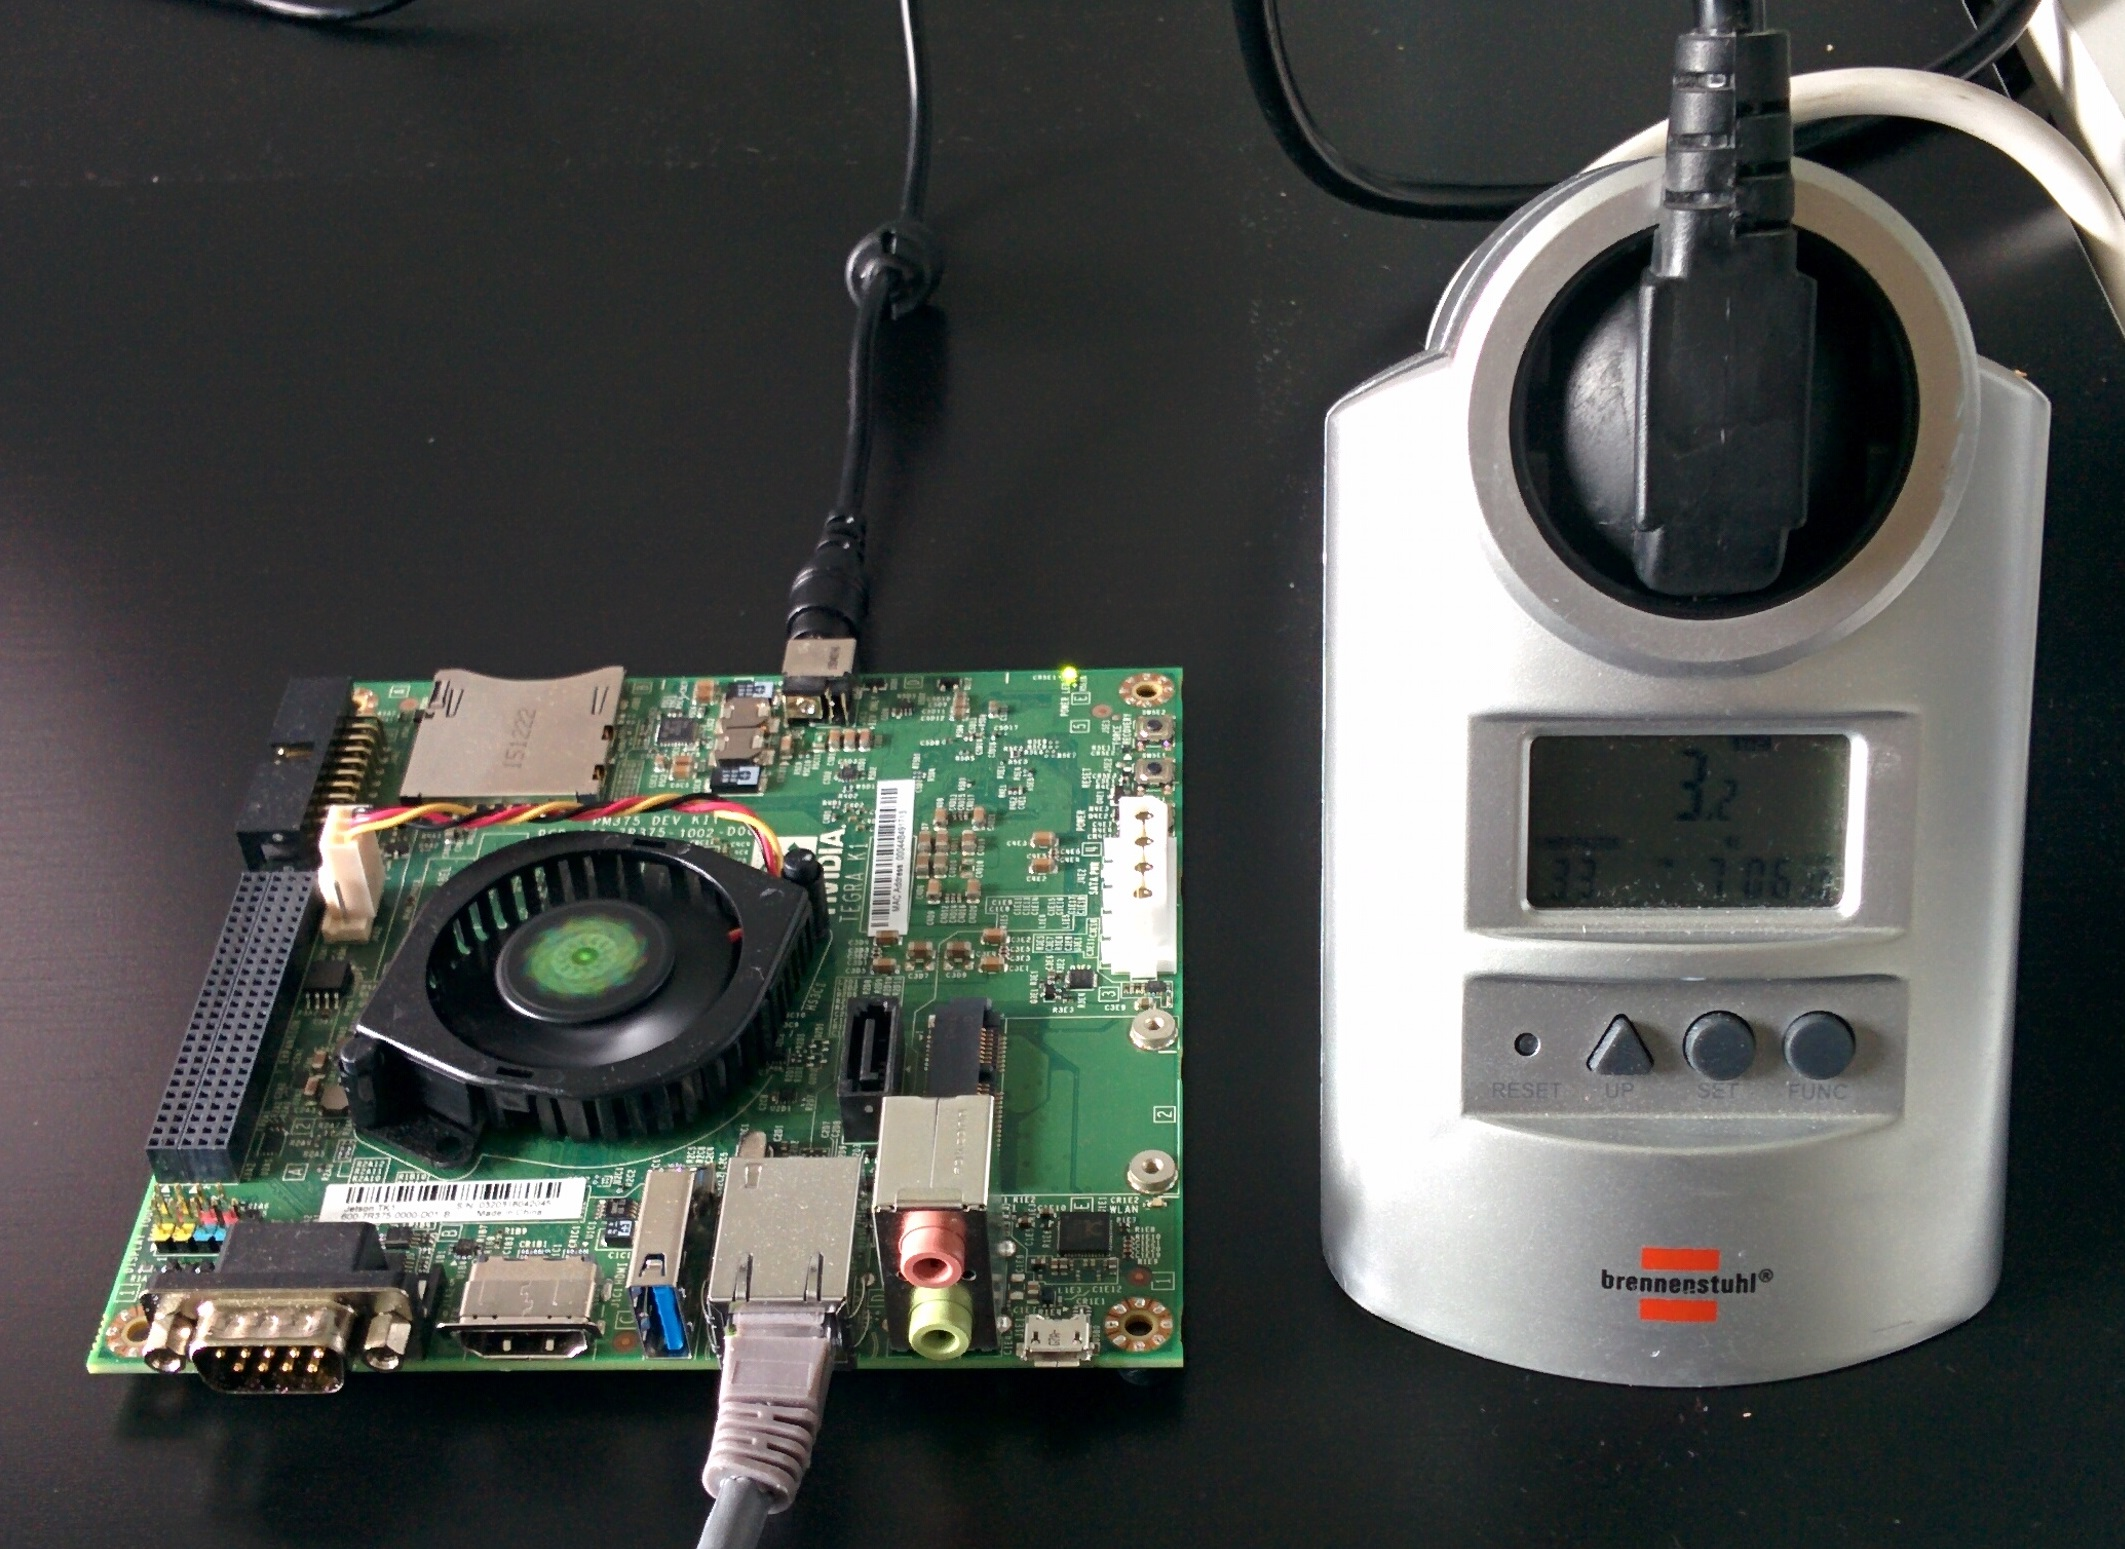
\includegraphics[width=\textwidth]{power/tk1.jpg}
\caption{Setup of the Tegra K1 board and the power meter.}
\label{tk1_photo}
\end{figure}

\subsection{TK1 CPU energy consumption}
Since the TK1 CPU is not particularly high performing a single all nearest neighbors search takes enough time to sample the power meter reading multiple times. The average of the power meter readings is $6.4 \pm 0.1 \unit{W}$. In this case we decide to ignore the power usage baseline of the board for two reasons: the first is that being very small (of the order of $\sim 1 \unit{W}$) does contribute little to the overall energy consumption, while the second is that the development board is a much simpler unit than a complete desktop computer and when running the KD-tree algorithm all its resources are dedicated to the task (contrary to the PC that might perform other requests from the operative system while the program is running on the GPU) and the whole power usage should be attributed to the program running.\\
After the generation of $5 \times 10^5$ random uniform distributed points and the build of the tree on those points, we measure the time needed for the TK1 CPU to perform an all nearest neighbors search. We perform the measure multiple times to verify the steadiness of the timing and the average result is $34.2 \pm 0.1 \unit{s}$. Therefore the energy consumed by the TK1 board to execute the search sequentially on one of its CPU cores is: $219 \pm 3 \unit{J/search}$.

\subsection{TK1 GPU energy consumption}
We repeat the measure on the board's GPU, since in this case the search is faster we can perform the measurement with different numbers of repetitions of the search: from 1 to 10 increasing by 1. The average power usage measured is $9.4 \pm 0.1 \unit{W}$, constant through all the repetitions.
The average time spent by the TK1 GPU to perform a search is $1.2 \pm 0.1 \unit{s}$. The energy consumption of the board while running the search on the GPU is then $11 \pm 1 \unit{J/search}$.

\section{Consumption comparisons}
The energy consumption results are very clear: among the setups evaluated the parallel GPU code is always more energy efficient than its sequential counterpart. When comparing the consumption of the desktop PC GPU board respect to the same machine CPU the parallel code only uses $\sim15\%$ of the energy required by the CPU to execute the sequential code. This fact demonstratesthat a specifically designed code not only can run faster than a more generic one but can also be more energy efficient. Moreover when applying the same GPU code with an even more specific hardware (for example the TK1) this efficiency margin increase further, in our setup by another $\sim20\%$.\\
The TK1 also shows another very desirable feature: while it is true that the raw performance on this chip are quite worse with respect to the full GPU board, they are still reasonable (although not enough to be considered for the HGCAL HLT) and, most importantly, they can be achieved with a minimal power usage of less than $10 \unit{W}$. This is a really crucial point, since such a low peak power usage allows to place several of those chips in a small volume where the heat dissipation can be easily achieved with low cost airflow mechanisms.\\
The above feature, alongside the low cost of these chips and their architecture that guarantees a general purpose usage with good performance could really make the System-on-a-Chip a valuable device for the future of the high energy physics data taking.
